\documentclass[conference]{IEEEtran}
\usepackage{IEEEpreamble}

\usepackage{booktabs}
\usepackage{blindtext}
\usepackage{sepnum}
\usepackage{url}
\usepackage{listings}
\usepackage{zi4}
\usepackage{minted}

\usepackage{tikz}

\newcommand{\urlcount}{2,127,284}
\newcommand{\xlscount}{249,376}
\newcommand{\urlcountunique}{292,043}

\lstset{
  basicstyle=\small\ttfamily
}

\begin{document}
%
% paper title
% can use linebreaks \\ within to get better formatting as desired
\title{\textsc{Fuse}: A Reproducible, Extendable, Internet-scale\\Corpus of Spreadsheets}

\author{
\IEEEauthorblockN{Titus Barik\IEEEauthorrefmark{1}\IEEEauthorrefmark{2}, Kevin Lubick\IEEEauthorrefmark{2}, Justin Smith\IEEEauthorrefmark{2}, John Slankas\IEEEauthorrefmark{2}, Emerson Murphy-Hill\IEEEauthorrefmark{2}}
\IEEEauthorblockA{\IEEEauthorrefmark{1}ABB Corporate Research, Raleigh, North Carolina, USA\\
\IEEEauthorrefmark{2}North Carolina State University, Raleigh, North Carolina USA\\
titus.barik@us.abb.com, \{kjlubick, jssmit11, jbslanka\}@ncsu.edu, emerson@csc.ncsu.edu
}}

\maketitle

\begin{abstract}
Spreadsheets are perhaps the most ubiquitous form of end-user programming software. This paper describes a corpus, called \textsc{Fuse}, containing 
\urlcount{} URLs (and their HTTP server responses) that return spreadsheets, and \xlscount{} unique spreadsheets, contained within a public web archive of over 26.83 billion pages. Obtained using nearly 60,000 hours of computation, the resulting corpus exhibits several useful properties over prior spreadsheet corpora, including reproducibility and extendability. Our corpus is unencumbered by any license agreements, available to all, and intended for wide usage by end-user software engineering researchers. In this paper, we detail the data and the spreadsheet extraction process, describe the data schema, and discuss the trade-offs of \textsc{Fuse} with other corpora.
\end{abstract}


\IEEEpeerreviewmaketitle

% Oops: we forgot to handle application/vnd.oasis.opendocument.spreadsheet.

% \textbf{Data papers}. We want to encourage researchers to share their data. Data papers should describe data sets curated by their authors and made available to others. They are expected to be at most 4 pages long and should address the following: description of the data, including its source; methodology used to gather it; description of the schema used to store it, and any limitations and/or challenges of this data set. The data should be made available at the time of submission of the paper for review, but will be considered confidential until publication of the paper. Further details about data papers are available on the conference website. 

% \begin{enumerate}
% \item Description of the data.
% \item Methodology used to gather it
% \item Description of the schema used to store it
% \item Limitations and Challenges of data set
% \end{enumerate}

\section{Introduction}

End-user programmers today constitute a broad class of users, including teachers, accountants, administrators, managers, research scientists, and even children~\cite{Ko2011}.
%
Although these users are typically not professional software developers, their roles routinely involve computational tasks that, in many ways, are similar to those of developers --- not just in activity, but also in their underlying cognitive demands on users~\cite{Blackwell2002}. 

Perhaps the most ubiquitous form~\cite{Scaffidi2005} of end-user programming software are \emph{spreadsheets}, a table-oriented visual interface that serves as the underlying model for the users' applications~\cite{Nardi1990}. \emph{Cells} within these tables are augmented with computation, such as expressions, functions and macros~\cite{Nardi1990}. 
This interplay between presentation and computation within the spreadsheet environment has garnered significant interest from the software engineering research community~\cite{Burnett2009}. 
Researchers have adopted techniques and approaches to studying errors~\cite{Pinzger2012}, code smells~\cite{Badame2012}, and debugging in spreadsheets~\cite{Powell2008}, similar to traditional programming environments. 

% \footnote{``Spreadsheets are not just tools for doing “what-if” analysis. They provide a specific data structure: a table. Most Excel users never enter a formula. They use Excel when they need a table. The gridlines are the most important feature of Excel.'' \url{http://www.joelonsoftware.com/items/2012/01/06.html}}.

To better understand end-user activities and design tools to assist end-users, researchers have responded by curating spreadsheet corpora to support spreadsheet studies~\cite{Fisher2005,Hermans2015,Chen2013}. This paper presents one such spreadsheet corpus, called \textsc{Fuse}, extracted from the over 26.83 billion web pages in the Common Crawl index. We believe that \textsc{Fuse} offers several useful traits not found in prior corpora; 
for example, \textsc{Fuse} is obtained in such a way that researchers can independently reproduce an identical corpus from source materials.

% http://www.felienne.com/archives/3634
% \begin{table}[!t]
% %% increase table row spacing, adjust to taste
% %\renewcommand{\arraystretch}{1.3}
% % if using array.sty, it might be a good idea to tweak the value of
% % \extrarowheight as needed to properly center the text within the cells
% \caption{Comparison of \textsc{Fuse} and other spreadsheet corpora\label{tab:corpora}}
% \centering
% %% Some packages, such as MDW tools, offer better commands for making tables
% %% than the plain LaTeX2e tabular which is used here.
% \begin{tabular}{llllll}
% \toprule
%  & \textbf{\textsc{Fuse}} & \textbf{EUSES} & \textbf{Enron} & \textbf{ClueWeb}\\
% \midrule
% Size ($n$) & 249,376 & 6,000 & 15,570 & 410,554\\
% Space (GB) & 87  & 0.64 & 23.3 & 110\\
% Access & All & Researchers & All & All\\
% Unique formulas & 894,361 & 84,004 & 784,380  & --\\
% Extendable & Yes & Yes & No & Yes\\
% Framework & Hadoop & Excel/VBA & Scantool & \textsc{--}\\
% Scalable & Yes & No & No & Yes\\
% Collection period & 2013-2014 & 2006 & 2006 & 2009\\
% Pri. origin & CC & Google & Enron & ClueWeb\\
% Binaries & Yes  & Yes & Yes & No\\
% Metadata & Yes & No & No & No\\
% Domains & 4,318 & - & - & 51,157\\
% Distinct functions & 219 & 209 & 139 & --\\
% \bottomrule
% \end{tabular}
% \end{table}



% TODO(tbarik): Just for reference. Remove for submission.
% The text height is \the\columnwidth -- should 252.0pt or 3.5in.


The contributions of this paper are two related datasets, which together constitute the \textsc{Fuse} spreadsheet corpus\footnote{The corpus metadata, spreadsheets, tools, and other documentation can be obtained at \url{http://go.barik.net/fuse}.}
:

\begin{itemize}
\item A \emph{Web Analysis} dataset of \urlcount{} URLs that return spreadsheet content, along with the full HTTP web server response, formatted as JSON records. This dataset is obtained by filtering through 26.83 billion HTTP responses within the Common Crawl archive.
\item A \emph{Binary Analysis} dataset of \xlscount{} spreadsheets, extracted from the 1.9 PB of raw data within the Common Crawl archives. For each spreadsheet, we have provided associated JSON metadata containing our analysis, which includes NLP token extraction and spreadsheet metrics.
\end{itemize}

  % \item A modular, open-source tool pipeline, implemented using MapReduce. This scalable tool can process over 1 million spreadsheets in under an hour.


% \begin{figure}[!t]
% \centering
% 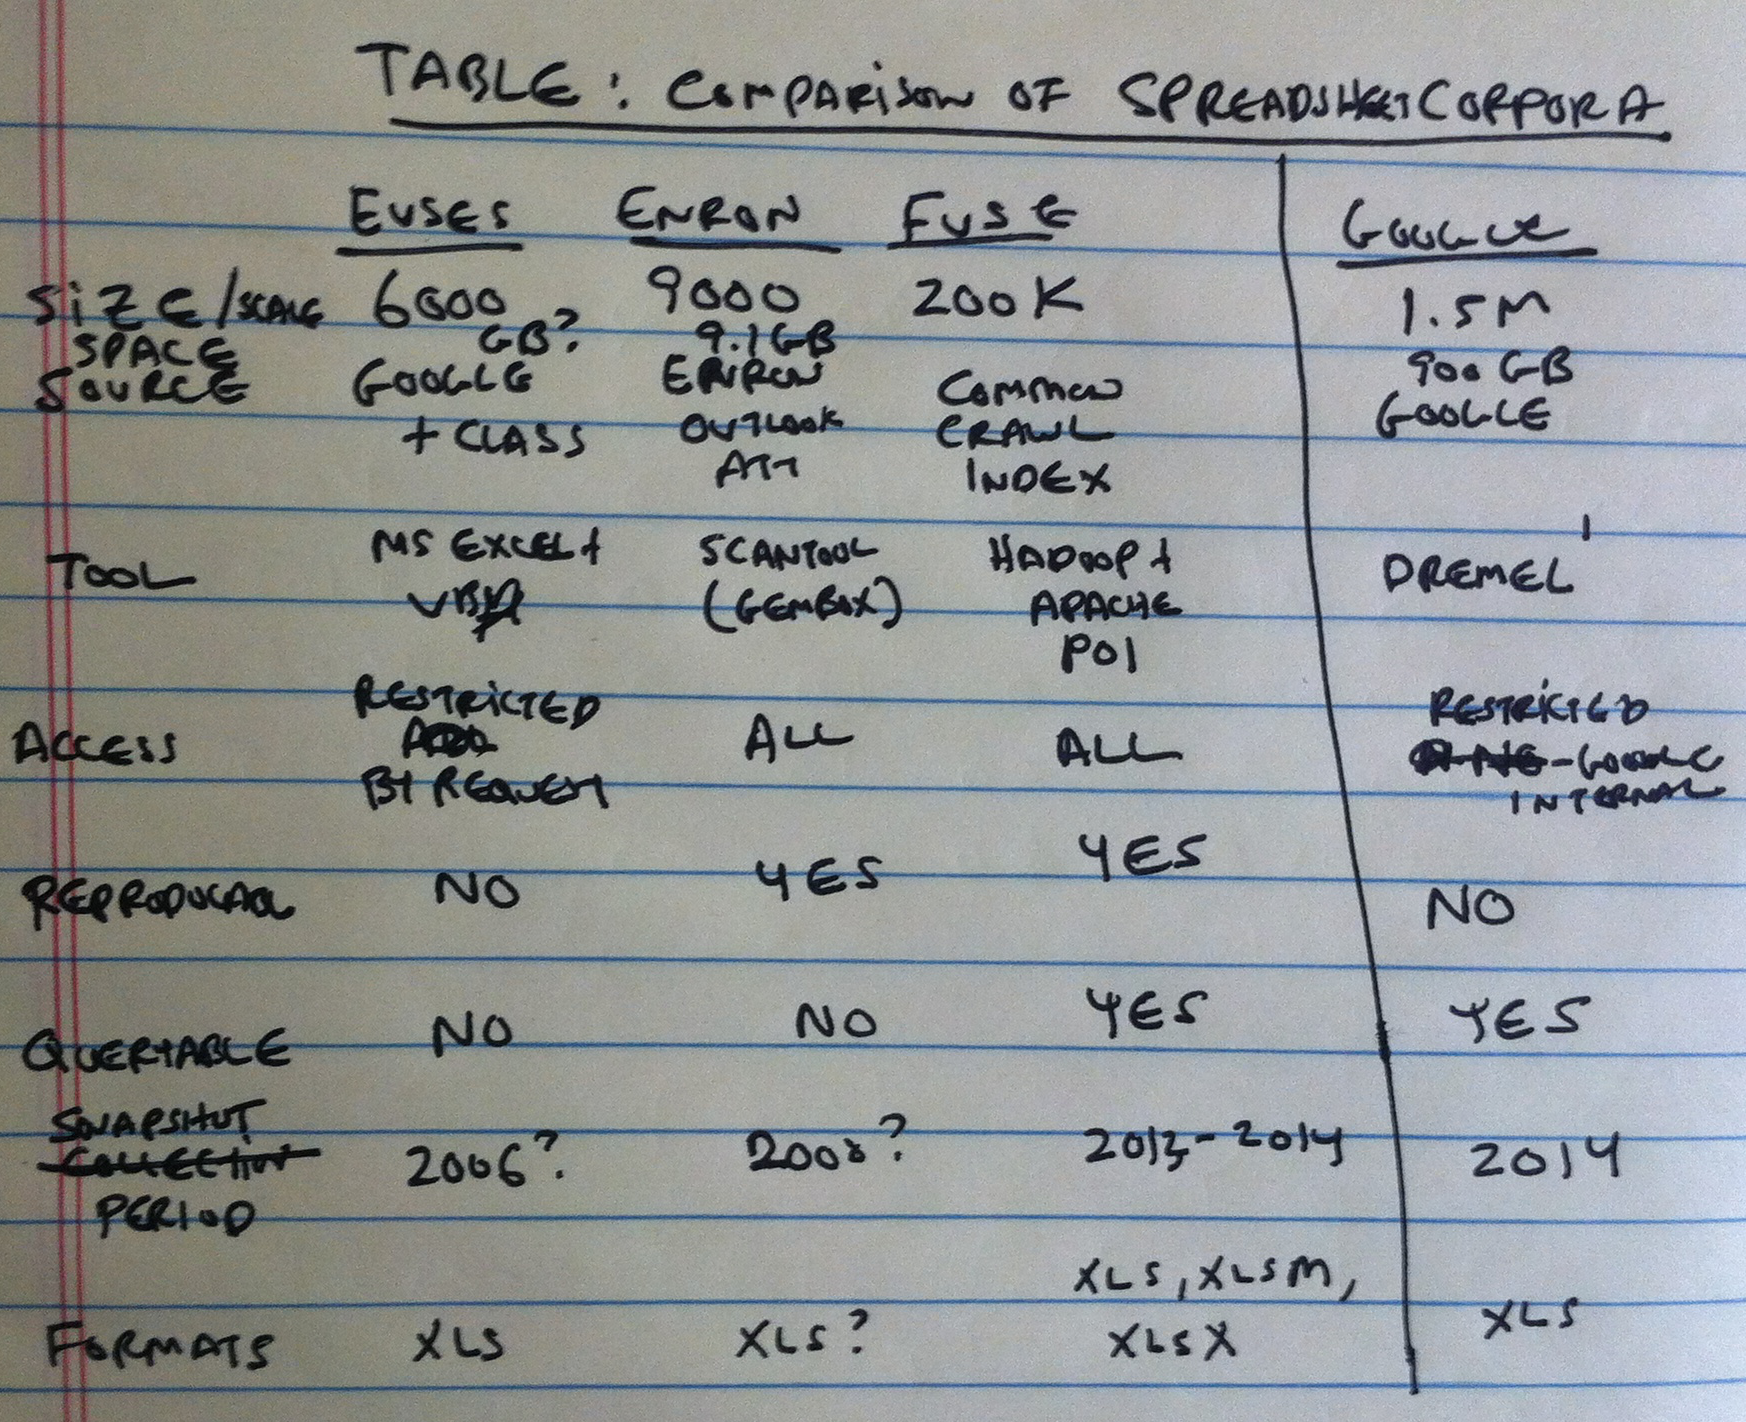
\includegraphics[width=\columnwidth]{corpora}
% \caption{Comparison matrix of available spreadsheet corpora. How does \textsc{Fuse} stack up?}
% \label{fig:corpora}
% \end{figure}


% Improve display of JSON files
% http://tex.aspcode.net/view/635399273629833626148902/how-to-improve-listings-display-of-json-files

% TODO(tbarik)
%  This WAT file is okay, but the corresponding WARC record is corrupt:
% Put an example of this issue in the methodology.
%  {"WARC-Date":"2014-09-22T12:11:35Z","WARC-Record-ID":"<urn:uuid:0d670ac1-319f-42b0-89bf-7c52dd51e1dd>","Content-Length":1385,"WARC-Target-URI":"http://www.medcom.dk/dwn1514.xls","WARC-Content-Type":"application/json","Content":{"Envelope":{"Format":"WARC","WARC-Header-Length":"350","Block-Digest":"sha1:6JCTYB2KGCZ5YX63EFLECRMXB4KUBOQB","Actual-Content-Length":"263","WARC-Header-Metadata":{"WARC-Type":"request","WARC-Date":"2014-09-22T12:11:35Z","WARC-Warcinfo-ID":"<urn:uuid:1c4997f8-bc87-4ade-8efd-47f4cb8ce2a6>","Content-Length":"263","WARC-Record-ID":"<urn:uuid:81815bbd-d47d-4755-8e41-d820a1d05043>","WARC-Target-URI":"http://www.medcom.dk/dwn1514.xls","WARC-IP-Address":"91.193.139.41","Content-Type":"application/http; msgtype=request"},"Payload-Metadata":{"Trailing-Slop-Length":"4","HTTP-Request-Metadata":{"Headers":{"Accept-Language":"en-us,en-gb,en;q=0.7,*;q=0.3","Host":"www.medcom.dk","Accept-Encoding":"x-gzip, gzip, deflate","User-Agent":"CCBot/2.0 (http://commoncrawl.org/faq/)","Accept":"text/html,application/xhtml+xml,application/xml;q=0.9,*/*;q=0.8"},"Headers-Length":"261","Entity-Length":"0","Entity-Trailing-Slop-Bytes":"0","Request-Message":{"Method":"GET","Version":"HTTP/1.0","Path":"/dwn1514.xls"},"Entity-Digest":"sha1:3I42H3S6NNFQ2MSVX7XZKYAYSCX5QBYJ"},"Actual-Content-Type":"application/http; msgtype=request"}},"Container":{"Compressed":true,"Gzip-Metadata":{"Footer-Length":"8","Deflate-Length":"418","Header-Length":"10","Inflated-CRC":"505390695","Inflated-Length":"617"},"Offset":"654053188","Filename":"CC-MAIN-20140914011217-00240-ip-10-234-18-248.ec2.internal.warc.gz"}},"WARC-Refers-To":"<urn:uuid:81815bbd-d47d-4755-8e41-d820a1d05043>","Path":"common-crawl/crawl-data/CC-MAIN-2014-41/segments/1410657137046.16/wat/CC-MAIN-20140914011217-00240-ip-10-234-18-248.ec2.internal.warc.wat.gz"}

\section{Description of Data}

\begin{figure}[!t]
\centering
% % Created by tikzDevice version 0.8.1 on 2015-02-23 21:41:07
% !TEX encoding = UTF-8 Unicode
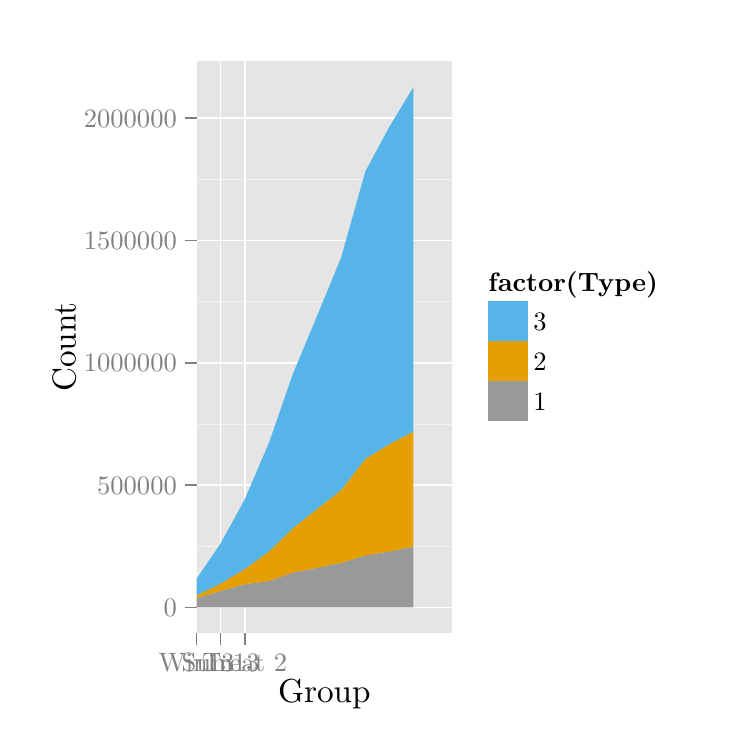
\begin{tikzpicture}[x=1pt,y=1pt]
\definecolor{fillColor}{RGB}{255,255,255}
\path[use as bounding box,fill=fillColor,fill opacity=0.00] (0,0) rectangle (252.94,252.94);
\begin{scope}
\path[clip] (  0.00,  0.00) rectangle (252.94,252.94);
\definecolor{drawColor}{RGB}{255,255,255}
\definecolor{fillColor}{RGB}{255,255,255}

\path[draw=drawColor,line width= 0.6pt,line join=round,line cap=round,fill=fillColor] (  0.00,  0.00) rectangle (252.94,252.95);
\end{scope}
\begin{scope}
\path[clip] ( 61.01, 34.03) rectangle (153.35,240.90);
\definecolor{fillColor}{gray}{0.90}

\path[fill=fillColor] ( 61.01, 34.03) rectangle (153.35,240.90);
\definecolor{drawColor}{gray}{0.95}

\path[draw=drawColor,line width= 0.3pt,line join=round] ( 61.01, 65.54) --
	(153.35, 65.54);

\path[draw=drawColor,line width= 0.3pt,line join=round] ( 61.01,109.74) --
	(153.35,109.74);

\path[draw=drawColor,line width= 0.3pt,line join=round] ( 61.01,153.94) --
	(153.35,153.94);

\path[draw=drawColor,line width= 0.3pt,line join=round] ( 61.01,198.14) --
	(153.35,198.14);
\definecolor{drawColor}{RGB}{255,255,255}

\path[draw=drawColor,line width= 0.6pt,line join=round] ( 61.01, 43.44) --
	(153.35, 43.44);

\path[draw=drawColor,line width= 0.6pt,line join=round] ( 61.01, 87.64) --
	(153.35, 87.64);

\path[draw=drawColor,line width= 0.6pt,line join=round] ( 61.01,131.84) --
	(153.35,131.84);

\path[draw=drawColor,line width= 0.6pt,line join=round] ( 61.01,176.04) --
	(153.35,176.04);

\path[draw=drawColor,line width= 0.6pt,line join=round] ( 61.01,220.25) --
	(153.35,220.25);

\path[draw=drawColor,line width= 0.6pt,line join=round] ( 61.01, 34.03) --
	( 61.01,240.90);

\path[draw=drawColor,line width= 0.6pt,line join=round] ( 69.73, 34.03) --
	( 69.73,240.90);

\path[draw=drawColor,line width= 0.6pt,line join=round] ( 78.44, 34.03) --
	( 78.44,240.90);
\definecolor{fillColor}{gray}{0.60}

\path[fill=fillColor] ( 61.01, 46.81) --
	( 69.73, 49.45) --
	( 78.44, 51.86) --
	( 87.15, 52.98) --
	( 95.86, 56.07) --
	(104.57, 57.80) --
	(113.28, 59.56) --
	(121.99, 62.25) --
	(130.70, 63.63) --
	(139.41, 65.48) --
	(139.41, 43.44) --
	(130.70, 43.44) --
	(121.99, 43.44) --
	(113.28, 43.44) --
	(104.57, 43.44) --
	( 95.86, 43.44) --
	( 87.15, 43.44) --
	( 78.44, 43.44) --
	( 69.73, 43.44) --
	( 61.01, 43.44) --
	cycle;
\definecolor{fillColor}{RGB}{230,159,0}

\path[fill=fillColor] ( 61.01, 47.78) --
	( 69.73, 52.08) --
	( 78.44, 57.34) --
	( 87.15, 63.63) --
	( 95.86, 72.15) --
	(104.57, 79.04) --
	(113.28, 85.87) --
	(121.99, 97.11) --
	(130.70,102.47) --
	(139.41,107.02) --
	(139.41, 65.48) --
	(130.70, 63.63) --
	(121.99, 62.25) --
	(113.28, 59.56) --
	(104.57, 57.80) --
	( 95.86, 56.07) --
	( 87.15, 52.98) --
	( 78.44, 51.86) --
	( 69.73, 49.45) --
	( 61.01, 46.81) --
	cycle;
\definecolor{fillColor}{RGB}{86,180,233}

\path[fill=fillColor] ( 61.01, 53.75) --
	( 69.73, 66.58) --
	( 78.44, 82.49) --
	( 87.15,102.81) --
	( 95.86,127.91) --
	(104.57,148.78) --
	(113.28,169.89) --
	(121.99,200.95) --
	(130.70,217.13) --
	(139.41,231.50) --
	(139.41,107.02) --
	(130.70,102.47) --
	(121.99, 97.11) --
	(113.28, 85.87) --
	(104.57, 79.04) --
	( 95.86, 72.15) --
	( 87.15, 63.63) --
	( 78.44, 57.34) --
	( 69.73, 52.08) --
	( 61.01, 47.78) --
	cycle;
\end{scope}
\begin{scope}
\path[clip] (  0.00,  0.00) rectangle (252.94,252.94);
\definecolor{drawColor}{gray}{0.50}

\node[text=drawColor,anchor=base east,inner sep=0pt, outer sep=0pt, scale=  0.96] at ( 53.90, 40.13) {0};

\node[text=drawColor,anchor=base east,inner sep=0pt, outer sep=0pt, scale=  0.96] at ( 53.90, 84.33) {500000};

\node[text=drawColor,anchor=base east,inner sep=0pt, outer sep=0pt, scale=  0.96] at ( 53.90,128.54) {1000000};

\node[text=drawColor,anchor=base east,inner sep=0pt, outer sep=0pt, scale=  0.96] at ( 53.90,172.74) {1500000};

\node[text=drawColor,anchor=base east,inner sep=0pt, outer sep=0pt, scale=  0.96] at ( 53.90,216.94) {2000000};
\end{scope}
\begin{scope}
\path[clip] (  0.00,  0.00) rectangle (252.94,252.94);
\definecolor{drawColor}{gray}{0.50}

\path[draw=drawColor,line width= 0.6pt,line join=round] ( 56.75, 43.44) --
	( 61.01, 43.44);

\path[draw=drawColor,line width= 0.6pt,line join=round] ( 56.75, 87.64) --
	( 61.01, 87.64);

\path[draw=drawColor,line width= 0.6pt,line join=round] ( 56.75,131.84) --
	( 61.01,131.84);

\path[draw=drawColor,line width= 0.6pt,line join=round] ( 56.75,176.04) --
	( 61.01,176.04);

\path[draw=drawColor,line width= 0.6pt,line join=round] ( 56.75,220.25) --
	( 61.01,220.25);
\end{scope}
\begin{scope}
\path[clip] (  0.00,  0.00) rectangle (252.94,252.94);
\definecolor{drawColor}{gray}{0.50}

\path[draw=drawColor,line width= 0.6pt,line join=round] ( 61.01, 29.77) --
	( 61.01, 34.03);

\path[draw=drawColor,line width= 0.6pt,line join=round] ( 69.73, 29.77) --
	( 69.73, 34.03);

\path[draw=drawColor,line width= 0.6pt,line join=round] ( 78.44, 29.77) --
	( 78.44, 34.03);
\end{scope}
\begin{scope}
\path[clip] (  0.00,  0.00) rectangle (252.94,252.94);
\definecolor{drawColor}{gray}{0.50}

\node[text=drawColor,anchor=base,inner sep=0pt, outer sep=0pt, scale=  0.96] at ( 61.01, 20.31) {Win13};

\node[text=drawColor,anchor=base,inner sep=0pt, outer sep=0pt, scale=  0.96] at ( 69.73, 20.31) {Sum13};

\node[text=drawColor,anchor=base,inner sep=0pt, outer sep=0pt, scale=  0.96] at ( 78.44, 20.31) {Treat 2};
\end{scope}
\begin{scope}
\path[clip] (  0.00,  0.00) rectangle (252.94,252.94);
\definecolor{drawColor}{RGB}{0,0,0}

\node[text=drawColor,anchor=base,inner sep=0pt, outer sep=0pt, scale=  1.20] at (107.18,  9.03) {Group};
\end{scope}
\begin{scope}
\path[clip] (  0.00,  0.00) rectangle (252.94,252.94);
\definecolor{drawColor}{RGB}{0,0,0}

\node[text=drawColor,rotate= 90.00,anchor=base,inner sep=0pt, outer sep=0pt, scale=  1.20] at ( 17.30,137.47) {Count};
\end{scope}
\begin{scope}
\path[clip] (  0.00,  0.00) rectangle (252.94,252.94);
\definecolor{fillColor}{RGB}{255,255,255}

\path[fill=fillColor] (162.22,106.40) rectangle (232.03,168.54);
\end{scope}
\begin{scope}
\path[clip] (  0.00,  0.00) rectangle (252.94,252.94);
\definecolor{drawColor}{RGB}{0,0,0}

\node[text=drawColor,anchor=base west,inner sep=0pt, outer sep=0pt, scale=  0.96] at (166.49,157.64) {\bfseries factor(Type)};
\end{scope}
\begin{scope}
\path[clip] (  0.00,  0.00) rectangle (252.94,252.94);
\definecolor{drawColor}{RGB}{255,255,255}
\definecolor{fillColor}{gray}{0.95}

\path[draw=drawColor,line width= 0.6pt,line join=round,line cap=round,fill=fillColor] (166.49,139.57) rectangle (180.94,154.03);
\end{scope}
\begin{scope}
\path[clip] (  0.00,  0.00) rectangle (252.94,252.94);
\definecolor{fillColor}{RGB}{86,180,233}

\path[fill=fillColor] (166.49,139.57) rectangle (180.94,154.03);

\path[] (166.49,139.57) --
	(180.94,154.03);
\end{scope}
\begin{scope}
\path[clip] (  0.00,  0.00) rectangle (252.94,252.94);
\definecolor{drawColor}{RGB}{255,255,255}
\definecolor{fillColor}{gray}{0.95}

\path[draw=drawColor,line width= 0.6pt,line join=round,line cap=round,fill=fillColor] (166.49,125.12) rectangle (180.94,139.57);
\end{scope}
\begin{scope}
\path[clip] (  0.00,  0.00) rectangle (252.94,252.94);
\definecolor{fillColor}{RGB}{230,159,0}

\path[fill=fillColor] (166.49,125.12) rectangle (180.94,139.57);

\path[] (166.49,125.12) --
	(180.94,139.57);
\end{scope}
\begin{scope}
\path[clip] (  0.00,  0.00) rectangle (252.94,252.94);
\definecolor{drawColor}{RGB}{255,255,255}
\definecolor{fillColor}{gray}{0.95}

\path[draw=drawColor,line width= 0.6pt,line join=round,line cap=round,fill=fillColor] (166.49,110.67) rectangle (180.94,125.12);
\end{scope}
\begin{scope}
\path[clip] (  0.00,  0.00) rectangle (252.94,252.94);
\definecolor{fillColor}{gray}{0.60}

\path[fill=fillColor] (166.49,110.67) rectangle (180.94,125.12);

\path[] (166.49,110.67) --
	(180.94,125.12);
\end{scope}
\begin{scope}
\path[clip] (  0.00,  0.00) rectangle (252.94,252.94);
\definecolor{drawColor}{RGB}{0,0,0}

\node[text=drawColor,anchor=base west,inner sep=0pt, outer sep=0pt, scale=  0.96] at (182.75,143.50) {3};
\end{scope}
\begin{scope}
\path[clip] (  0.00,  0.00) rectangle (252.94,252.94);
\definecolor{drawColor}{RGB}{0,0,0}

\node[text=drawColor,anchor=base west,inner sep=0pt, outer sep=0pt, scale=  0.96] at (182.75,129.04) {2};
\end{scope}
\begin{scope}
\path[clip] (  0.00,  0.00) rectangle (252.94,252.94);
\definecolor{drawColor}{RGB}{0,0,0}

\node[text=drawColor,anchor=base west,inner sep=0pt, outer sep=0pt, scale=  0.96] at (182.75,114.59) {1};
\end{scope}
\end{tikzpicture}

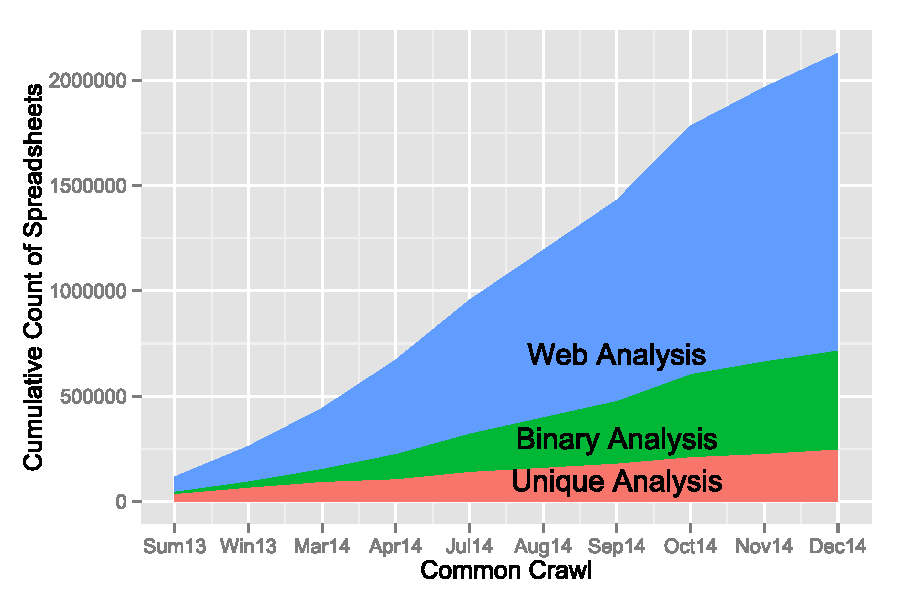
\includegraphics[width=\columnwidth]{figures/stack}
\caption{Cumulative count of spreadsheets obtained with each additional crawl. Web Analysis contains all URLs and associated HTTP server responses, while the Binary Analysis contains the actual spreadsheets for subset of the Web Analysis, archived within Common Crawl.\label{fig:rplot}}
\end{figure}

% TODO(tbarik): Kevin's POI Analysis is not available. We need the counts for the figure. Looks like the count is 680876.
\begin{figure*}[!t]
\centering
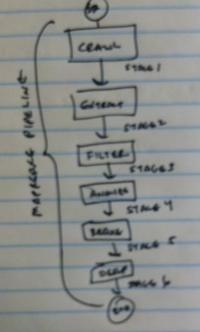
\includegraphics[width=\linewidth]{pipeline}
\caption{The MapReduce pipeline for extracting spreadsheets and associated spreadsheet analysis metadata from Common Crawl.\label{fig:mrpipeline}}
\end{figure*}


The Common Crawl\footnote{\url{http://commoncrawl.org}} non-profit organization is dedicated to providing a copy of the Internet, and democratizing the web crawl data so that it is accessible to everyone. 
%
Of specific interest to us is that the corpus contains not only the HTTP responses of web pages, but also the raw content of each of these resources, including binaries. It is from these monthly Web crawls that we extract and make available spreadsheets and corresponding metadata, augmented with our analysis, and tailored to researchers.

% The result, \textsc{Fuse}, is characterized through two, hierarchical datasets: 1) a Web Analysis dataset that contains the target URL and HTTP response headers of spreadsheets on the Web, and 2) a corpus that captures the associated spreadsheets for a subset of those URLs, described through metadata using our analysis tools, and 3) a corpus of unique spreadsheets extracted from the Web, where the binary content itself is primarily of interest.

The result, \textsc{Fuse}, is characterized through two, hierarchical datasets (Figure~\ref{fig:rplot}): a Web Analysis dataset, and a Binary Analysis dataset.

%TODO: What is this layer for?? Why is it not reproducible?
% 627,831 .org 2,127,284 (29.5\%)
% 589.928 .com 2,127,284 (27.7\%)
\textbf{Web Analysis:} This dataset contains \urlcount{} spreadsheet-related URLs and HTTP responses. 292,043 of these responses point to a unique URL, and the top domain is \texttt{.org} (29.5\%), followed by \texttt{.gov} (27.7\%). The analysis contains 6,316 distinct domain names. Unfortunately, relying solely on Web Analysis for spreadsheets will not result in a reproducible corpus, as the Internet is always in flux.

% \textbf{Binary Analysis Layer:} 719,223 of the records in the web analysis layer have valid spreadsheet content stored alongside the record Web Analysis layer --- this layer is stable because each crawl represents a fixed snapshot in time. Having content information, we find that URLs are not necessarily canonical. For example, we found 32,325 URIs in the corpora refer to more than one spreadsheet, which changes over time.

% 35,325, the largest of which change 61 times.
% Only propagated 589 times, and that the highest number of spreadsheets is only presented across 3 domains.

\textbf{Binary Analysis:}  To address the limitations of Web Analysis, the Binary Analysis dataset contains \xlscount{} unique spreadsheets, extracted directly from the raw data contained within Common Crawl archives, rather than the Internet. Since each monthly Common Crawl archive is a permanent snapshot in time, Binary Analysis is always reproducible.

Analyzing this layer, we discovered that \texttt{IF} is the most frequently used function, found in 17.8\% of all formula cells, giving evidence that spreadsheets require non-trivial computation. We also discovered that \texttt{=SUM(R[[-3]C:R[-1]C)} is the most common formula, in which a cell is the sum of the three cells to its left, and that it appears in 1,322 spreadsheets. In contrast with domain specific corpora, such as Enron, our general spreadsheet corpora has fewer formulas. Interestingly, only 7.00\% of our spreadsheets contain any formula, as opposed to 59.4\% of Enron spreadsheets, which is consistent with anecdotal findings of the Excel team.\footnote{Joel Spolsky writes, ``Everybody thought of Excel as a financial modeling application, [but] we visited dozens of Excel customers, and did not see anyone using Excel to actually perform what you would call `calculations.' Almost all of them were using Excel because it was a convenient way to create a table.'' --- \url{http://www.joelonsoftware.com/items/2012/01/06.html}}\\

% 14782 -> 2127279 (6.95\%)
% 8673 -> 14,600 (59.4\%)


% second most common
% across 1322 spreadsheets
% 1210 had  SUM(R[[-2]C:R[-1]C)  

This analysis hierarchy has several properties desirable to researchers, the first of which is reproducibility.
In Web Analysis, an independent researcher should always obtain the same set of spreadsheet-related URLs, provided they use the same spreadsheet detection heuristic.
Because the spreadsheets from Binary Analysis are obtained from content embedded in the Common Crawl corpus, these too are static, reproducible resources. A second property of our corpus is that it is open to extension, without sacrificing reproducibility. When Common Crawl releases a new dataset, these crawls can be incrementally incorporated into \textsc{Fuse}. A third useful property our corpus is related not to the data itself, but to its broader ecosystem: \textsc{Fuse} is unencumbered by any licensing requirements, available to all, and includes a scalable, open source toolchain.


% \begin{table}[!t]
% \caption{Top 10 Public-Suffixes\label{tab:suffix}}
% \centering
% \begin{tabular}{ll}
% \toprule
% Description & Frequency\\
% \midrule
% .gov & 250,21X\\
% .org & 171,845\\
% .com & 112,573\\
% .edu & 63,572\\
% .gov.au & 43,490\\
% .pa.us & 7,621\\
% .net & 7,409\\
% .mn.us & 4,641\\
% .ac.uk & 3,423\\ 
% .ca.us & 3,003 \\
% \bottomrule
% \end{tabular}
% \end{table}

% The top 10 domains from which Common Crawl spreadsheets were obtained is shown in Table~\ref{tab:suffix}. In total, we obtained 4,381 unique domains. In Common Crawl, spreadsheets are most frequently obtained from government-related sites. 143135 spreadsheets alone come from a single domain, \url{census.gov}.

% 4,381 domains. After dedup, 4,342.

% \begin{table}[!t]
% %% increase table row spacing, adjust to taste
% %\renewcommand{\arraystretch}{1.3}
% % if using array.sty, it might be a good idea to tweak the value of
% % \extrarowheight as needed to properly center the text within the cells
% \centering
% \label{tab:selectedFunctions}
% \caption{Selected Functions with counts per 1000 formula cells}
% \begin{tabular}{lllll}
% \toprule
%  & \textbf{\textsc{Fuse}} & \textbf{Enron} & \textbf{EUSES}\\
% \midrule
% IF & 178.8 & 157.3 & 166.8\\
% + (operator) & 166.4 & 173.7 & 167.6\\
% SUM & 87.7 & 63.7 & 153.6\\
% ISBLANK & 57.8 & 0.6 & 27.4\\
% VLOOKUP & 30.8 & 55.8 & 12.2\\
% HLOOKUP & 9.5 & 2.1 & 1.4\\
% AVERAGE & 32.0 & 8.1 & 7.9\\
% AND & 6.6 & 16.0 & 21.7\\
% NOT & 5.5 & 0.1 & 1.9\\
% \bottomrule
% \end{tabular}
% \end{table}

% \begin{table}[!t]
% \caption{Spreadsheet Classification\label{tab:ccrawl}}
% \centering
% \begin{tabular}{lll}
% \toprule
% \textbf{Category} & \textbf{\textsc{Fuse}} & \textbf{EUSES}\\
% \midrule
% Database & 4518 & 720\\
% Finance & 3058 & 780\\
% Grade & 2915 & 731\\
% Homework & 61 & 682\\
% Inventory & 2243 & 756\\
% Model & 2143 & 966\\
% \bottomrule
% \end{tabular}
% \end{table}

% we will briefly highlight the function counts found in Table II.
% This table demonstrates how the three corpora differ in composition.
% The Enron set, being mostly financial computation makes extensive use of commands such as VLOOKUP, where as the \textsc{Fuse} spreadsheets focus on string manipulation (ISBLANK) and simple calculations (AVERAGE).
% Surprisingly, the distributions differ between EUSES and \textsc{Fuse}, despite the two corpora being collected in similar ways.  
% No one corpus is sufficient for all possible end-user research, but we believe our extendable, scalable approach will give a wide variety for researchers now, and as it grows over the coming years.

\section{Methodology}

% This section describes our approach to extracting spreadsheets and their associated data from Common Crawl.

% Web pages: 26.83 billion.
% Petabytes: 1.9 PB
% Packed: 423.8 TB.

The Common Crawl is available as a public data set on Amazon, and crawl data is stored on Simple Storage Service (S3) as a set of WARC (Web ARCive) files, which store the raw crawl data, and a corresponding WAT file, which stores the web crawler metadata for the given WARC file. Essentially, each WAT file contains JSON-formatted records that act as an index into the WARC raw data. That is, each record contains a globally unique identifier, which we call a \texttt{WARC-Record-ID}, and a reference to a WARC filename, offset, and length. S3 supports downloading segments of files in this way.

We considered spreadsheets from the period of Summer 2013 through December 2014, which consists of 26.83 billion web pages, compressed as 423.8 TB (1.9 PB uncompressed). To support parallelization, this data is split into 481,427 segments, such that different machines can independently compute a segment. Extracting such a corpus from a single desktop machine is computationally intractable, and thus we extracted the spreadsheets using the Amazon Elastic MapReduce service.

% \footnote{The \emph{actual time} to completion is actually inconsequential. Since our pipeline is embarrassingly parallel, one need only choose an arbitrary time constraint under which they wish to complete the work, then provising an inversely proportional number of vCPUs to meet the deadline. In practice, we restricted our pipeline to slightly less than 1,600 vCPUs, for a total cost of approximately \$2,500 USD.}

 
% TODO(tbarik): Copy Mixin and JsonMerge, not shown, but utility tool to easily copy sets and merge them.

\subsection{Hadoop MapReduce Pipeline}

Figure~\ref{fig:mrpipeline} illustrates our MapReduce framework, which consists of five stages that comprise a pipeline. For each stage in the framework, we compute the cost in terms of normalized instance hours. The total hours correspond to the approximate amount of time that it would take for a 1 vCPU, 1.7 GiB machine to complete the task --- in other words, roughly comparable to a single end-user desktop machine.  Although researchers do not need to use our pipeline to reproduce our results, our framework already contains the necessary MapReduce scaffolding, such as task scheduling code, as well as Java libraries, to support distributed analysis.

\subsubsection{Match} 

This stage required that we traverse every JSON-formatted URL and HTTP response in the 481,427 WAT segments and match spreadsheet-related records. First, we checked if the HTTP response payload \texttt{Content-Type} field corresponded to one of seven spreadsheet MIME types as supported by Microsoft Excel.\footnote{\url{https://technet.microsoft.com/en-us/library/ee309278.aspx}} However, some records contained a generic binary \texttt{Content-Type} of \texttt{application/octet-stream}, in which case \texttt{Content-Disposition} was checked via a file pattern matching ``\texttt{.xls*}''. If either of these conditions were true, we saved the record using the \texttt{WARC-Record-ID} as the key. This is a heuristic process because cannot know for sure that a record is actually a spreadsheet until we inspect the extracted file. This key identified the file throughout the pipeline. After filtering through some 26.83 billion records, we identified 2,127,284 candidate spreadsheets. This stage, the most computationally expensive in the pipeline, required approximately 55,000 hours to process.

\subsubsection{Extract} 

The extract stage loaded the 2,127,284 candidate spreadsheets records. Using the \texttt{Filename}, \texttt{Offset}, and \texttt{Deflate-Length} fields of the record, the corresponding WAT record was extracted into memory. The WARC record was then stripped of its header information (e.g., the HTTP response), and the remaining content was saved to S3, again using the \texttt{WARC-Record-ID} from the WAT file as the key. Theoretically, this process should yield the same number of records as crawl stage; however, five records had corrupted \texttt{gzip} entries, yielding 2,127,279 candidate spreadsheets. This stage required approximately 1,000 hours to complete.

\subsubsection{Filter} 

The filter stage checks the extracted file and tags those that are actually spreadsheets. Using Apache Tika's built-in MimeType detector was used to return the actual Content-Type of the file. If this result was one of the spreadsheet content types, the record was retained. During this stage, we also computed the length (in bytes) of the spreadsheet, identified the most appropriate file extension (e.g., ``\texttt{.xlsx}''), and generated a SHA-1 digest of the spreadsheet content.  At this stage, 719,223 spreadsheets were retained in the pipeline, although many of these may be duplicates. This stage required 420 normalized instance hours to complete.

\subsubsection{Plugins} 

The fourth stage of the pipeline is actually a meta-stage, in which researchers can augment the framework with their own analysis using plugins. For our corpus, we augmented the JSON document with three plugins: \texttt{InternetDomain}, which uses the Google guava library to extracts domain-related information from the \texttt{WARC-Target-URI}; Apache POI, which obtains metrics on the content of the spreadsheets, such as the use of functions; and LingPipe, which extracts language-related information from the spreadsheet. These JSON records were all saved to S3 by their \texttt{WARC-Record-ID}. For various reasons, not all APIs can analyze all spreadsheets, even when they open in Microsoft Excel. This stage required about 300 normalized instance hours per plugin. Researchers wishing to build on our approach will be able to insert their own plugins at this stage, without having to recompute the first three stages, saving research time and effort. For convenience, we also retroactively ran the \texttt{InternetDomain} plugin on the JSON output from the \texttt{Match} stage to generate the Web Analysis dataset.

\subsubsection{Merge} 

The merge stage simply takes the resulting JSON files from all previous stages and combines them with the original WAT record to facilitate downstream analysis. The stage required approximately 130 normalized instance hours for each plugin. The output of merge, combined with the spreadsheets from the filter stage, comprise the Binary Analysis dataset.

\subsection{Local Operations}

% Finally, we eliminate any duplicate spreadsheets by removing records based upon match SHA-1 hash values where the record I'd is not the lowest value.

We compute a SHA-1 hash of the records from Binary Analysis, from which we perform a local (non-MapReduce), deterministic de-duplication operation. The result of this operation is 249,376 unique spreadsheets. Locally, we also converted all JSON documents \textsc{Fuse} to MongoDB format.


% https://publicsuffix.org/list/

% sebastien paper for other metrics a look inside common crawl
% http://blog.commoncrawl.org/2013/08/a-look-inside-common-crawls-210tb-2012-web-corpus/
% domain parsing is done using 

% https://publicsuffix.org/

% http://www.statmethods.net/advgraphs/images/ggplotdensity.png


\section{Data Schema}
\label{sec:schema}

% TODO(tbarik):
% Size of uncompressed, deduped binaries: 22 GB (22937824).
% Size of uncompressed, full binaries: 82 GB (85358856).

The most relevant elements from the Common Crawl WARC record are \texttt{WARC-Target-URI}, that is, the URL from which the spreadsheet and downloaded, and \texttt{Container}, which indicates the Common Crawl file and offset used to extract the spreadsheet from the crawl. The \texttt{WARC-Date} element may also be of interest, since it contains the time and date of the access. Using the \texttt{Content-Disposition} element, one can often extract the original spreadsheet file name.

The Apache Tika JSON element contains four fields, which include the \texttt{MIME} type, best-guess file extension, a SHA-1 signature, and the length in bytes of the spreadsheet:

\usemintedstyle{borland}
\begin{minted}{json}
{
  "Tika": {
      "Tika-Content-Type": 
         "application/vnd.ms-excel",
      "Tika-Extension": ".xls",
      "Digest": "sha1:...",
      "Length": 5123
  }
}
\end{minted}

The \texttt{InternetDomain} element is useful for analysis relating to the origin of a spreadsheet. It uses the \texttt{WARC-Target-URI} and extracts the host, the top private domain, and a public suffix\footnote{\url{https://publicsuffix.org/}}:

\begin{minted}{json}
{
  "WARC-Target-URI": 
      "http://www.example.org/results/test.xls",
  "InternetDomainName": {
    "Host": "www.example.org",    
    "Top-Private-Domain": "example.org",    
    "Public-Suffix": "org"
  }
}
\end{minted}

Next, we also provide an Alias-i \texttt{LingPipe} element, which extracts the token stream from spreadsheets, lowercases the tokens, removes English stop words (such as `a' or `the'), and filters out non-words (such as numbers). Again, the representation of this is simple:

\begin{minted}{json}
{
  "LingPipe": {    
    "Tokens": [
      "finance",      
      "city"      
    ]
  }
}
\end{minted}

Finally, to get a high-level overview of the content of the spreadsheets, we used Apache POI (namespace, \texttt{POI}) to gather spreadsheet metrics. There are over 450 such metrics, which include the number of times a given Excel function (such as \texttt{SUM} or \texttt{VLOOKUP}) is used, the total number of input cells (i.e. cells that are not formulas), the number of numeric input cells, and the most common formula used.

% The metadata file can be downloaded from HERE, unzipped, and then loaded into mongoDB\footnote{https://www.mongodb.org/} using the following command:
% \texttt{mongoimport --db spreadsheets --collection fuse --file fuse.metadata.json}

% Standard mongoDB queries can then be done on the analysis, such as 
% \begin{lstlisting}
% db.fuse.aggregate(
%     { "$match": 
%       {"Tika.Length" : { $gt: 1000000 } } },
%     { "$group": 
%       {"_id": "Big Spreadsheets",
%  "count": {"$sum": 1} } })
% \end{lstlisting}
% which counts how many spreadsheets are larger than 1 MB.


% The metadata we collected for the indices was largely influenced by the summary statistics presented in \cite{Fisher2005}.  
% For each spreadsheet, there are over 450 entries, so we will not list them all here.
% In general, the entries summarize the contents of the cells.
% To list a few examples, the number of times a given Excel function (such as \texttt{SUM} or \texttt{VLOOKUP}) is used, the total number of input or data cells, the number of numeric input cells, the number of formulas used more than 50 times, the most common formula used, etc.


% aws s3 ls --recursive s3://aws-publicdatasets/common-crawl/crawl-data/CC-MAIN-2014-10/segments | awk '$4 ~ /wat/ {print $4}' > wat.summer2013.path

% http://blogs.msdn.com/b/vsofficedeveloper/archive/2008/05/08/office-2007-open-xml-mime-types.aspx

% \section{Description of Spreadsheet Corpus}

% Using the data schema from Section~\ref{sec:schema}, and high-level numbers from the MapReduce pipeline, we can now characterize some of the interesting features in the dataset.

% \begin{table}[!t]
% \caption{Common Crawl Archive\label{tab:carchive}}
% \centering
% \begin{tabular}{lll}
% \toprule
% Description & TB & Yield\\
% \midrule
% Summer 2013 & 30.6 & 42.14\%\\
% Winter 2013 & 35.1 & 33.46\% \\
% March 2014 & 36.4 & \\
% April 2014 & 41.2 & \\
% July 2014 & 59.2 & \\
% August 2014 & 46.6 & \\
% September 2014 & 48.9 & \\
% October 2014 & 59.1 & \\
% November 2014 & 31.4 & \\
% December 2014 & 35.2 & \\
% \bottomrule
% \end{tabular}
% \end{table}

% \subsection{Public Suffixes}


% What domains are represented in the corpus?

% \begin{lstlisting}
% db.s.aggregate(
%     { "$project": 
%       {"InternetDomainName.Public-Suffix" : true } },
%     { "$group": 
%       {"_id": "$InternetDomainName.Public-Suffix", "count": {"$sum": 1} } },
%     { "$sort": { "count" : -1 } },
%     { "$limit": 10 }
% )
% \end{lstlisting}

% TLD bias: http://w3techs.com/technologies/overview/top_level_domain/all


% FOR SDL: topleveldomain

% absfreq, relfreq
% census.gov, 143135
% triathlon.org, 106486
% amamanualofstyle.com, 45118
% abs.gov.au, 42941
% utah.gov, 22242
% ohio.gov, 16739
% usda.gov, 13016
% worldbank.org, 11062
% theahl.com, 10350
% eia.gov, 8216

% \noindent\textbf{RQ: How many domains are represented?}



% TODO(tbarik): Make sure all MongoDB queries refer to the database the same way: fuse.

% how canonical are urls?

% not very

% db.s.aggregate(
%     { "$project": {"Tika.Digest": true, "WARC-Target-URI": true } },
%     { "$group": { "_id": { uri: "$WARC-Target-URI", sha: "$Tika.Digest" }, count: { "$sum": 1 } } },    
%     { "$group": { "_id": { uri: "$_id.uri" }, count: { "$sum": 1 } } },
%     { "$match": { "count" : { "$gte" : 2 } } },
%     { "$sort": { "count" : -1 } }  
% )


% euses and cc overlap
% sha1:24af0f8d6a5a18a44150a6b56587582546a0ba71  (1)
%   Inventory control form www.edu.edu
%    ./inventory/processed/InventoryControlForm.xls
% sha1:70cc5c391b4e439c61e003f0c01ea573fcea544b (3/but all same)
%     ncdenr.org
%     ./modeling/processed/labrates050104.xls
% sha1:9992cd834d4824cbb05c26b0ffcecff04509334c
%     naaccr.org
%     ./grades/processed/naaccr9a.xls
% sha1:9a09b5a28eb4faf6516ddac8aaf7c90eddc47090
%     http://www.courts.delaware.gov/forms/download.aspx?ID=21098
%     http://www.courts.delaware.gov/forms/download.aspx?id=21098
%     ./financial/processed/finanacial%20sheet.xls
% sha1:d903ce9171061b482d92aa78bb2e60404ab16732
%     nigc.gov
%     ./inventory/processed/TableInventorySlipWorksheet.xls    

% Media Type

% application/vnd.ms-excel, 238673
% application/vnd.openxmlformats-officedocument.spreadsheetml.sheet, 10555
% application/vnd.openxmlformats-officedocument.spreadsheetml.template, 148

% all zero:
% application/vnd.ms-excel.sheet.macroEnabled.12
% application/vnd.ms-excel.template.macroEnabled.12
% application/vnd.ms-excel.addin.macroEnabled.12
% application/vnd.ms-excel.sheet.binary.macroEnabled.12

% RQ: How much can you trust HTTP headers?
% RQ: Train a text classifier to identify topicality.
% RQ: Evolution of spreadsheets


% Breakdown of analysis:
%db.spreadsheet.aggregate(
%    { "$project": 
%      {"Summary.errorNotification" : true } },
%    { "$group": 
%      {"_id": "$Summary.errorNotification", "count": {"$sum": 1} } },
%    { "$sort": { "count" : -1 } },
%    { "$limit": 10 })

% "OK", 220760
% "BIFF5",  17643 
% "OTHER", 10782 
% "CORRUPT",129
% "ENCRYPTED",  62 

%	db.fuse.aggregate(
%    { "$group": 
%      {"_id": "Input Cells", "count": {"$sum": "$totalInputCells"} } })
% Total Input cells: 357210294

%	db.fuse.aggregate(
%    { "$group": 
%      {"_id": "Total Formula Cells", "count": {"$sum": "$totalFormulas"} } })
% Total Formula cells: 10776903
% some ideas for things to show
% http://blog.commoncrawl.org/2012/05/

% Total Non-empty cells: 357210294 + 10776903 = 367987197
% Average non-empty cells per workbook: 367987197/220760 = 1667

%db.fuse.aggregate([
%	{ $match: { totalFormulas: { "$gt": 0}}},
%    { "$group": 
%      {"_id": "Workbooks with Formulas", "count": {"$sum": 1} } }])
% Number of workbooks with formulas: 14782

% Number of formulas/workbook with formulas: 10776903/ 14782 = 729

% Number of unique formulas: 894361

% Number of unique formulas/workbook with formulas: 894361/ 14782 = 60

% Number of different functions used: 219

%db.fuse.aggregate(
%    { "$group": 
%      {"_id": "Total Sheets", "count": {"$sum": "$numSheets"} } })
% Total Sheets: 346247

%db.fuse.aggregate(
%	{ "$group": 
%      {"_id": "Maximum Sheets", "count": {"$max": "$numSheets"} } })
% Maximum number of sheets: 147

%>  db.fuse.aggregate({ "$group":{"_id": "Total countAVERAGEIF Cells", "count": {"$sum": "$countAVERAGEIF"} } })
%{ "_id" : "Total countAVERAGEIF Cells", "count" : 775 }
%>  db.fuse.aggregate({ "$group":{"_id": "Total countAVERAGEIFS Cells", "count": {"$sum": "$countAVERAGEIFS"} } })
%{ "_id" : "Total countAVERAGEIFS Cells", "count" : 162 }
%>  db.fuse.aggregate({ "$group":{"_id": "Total countCOUNTIF Cells", "count": {"$sum": "$countCOUNTIF"} } })
%{ "_id" : "Total countCOUNTIF Cells", "count" : 51239 }
%>  db.fuse.aggregate({ "$group":{"_id": "Total countCOUNTIFS Cells", "count": {"$sum": "$countCOUNTIFS"} } })
%{ "_id" : "Total countCOUNTIFS Cells", "count" : 1249 }
%>  db.fuse.aggregate({ "$group":{"_id": "Total countIF Cells", "count": {"$sum": "$countIF"} } })
%{ "_id" : "Total countIF Cells", "count" : 2496350 }
%>  db.fuse.aggregate({ "$group":{"_id": "Total countIFERROR Cells", "count": {"$sum": "$countIFERROR"} } })
%{ "_id" : "Total countIFERROR Cells", "count" : 181976 }
%>  db.fuse.aggregate({ "$group":{"_id": "Total countIFNA Cells", "count": {"$sum": "$countIFNA"} } })
%{ "_id" : "Total countIFNA Cells", "count" : 0 }
%>  db.fuse.aggregate({ "$group":{"_id": "Total countSUMIF Cells", "count": {"$sum": "$countSUMIF"} } })
%{ "_id" : "Total countSUMIF Cells", "count" : 94978 }
%>  db.fuse.aggregate({ "$group":{"_id": "Total countSUMIFS Cells", "count": {"$sum": "$countSUMIFS"} } })
%{ "_id" : "Total countSUMIFS Cells", "count" : 239 }

% \section{Kevin's Crap}

% Programming in spreadsheets:

% 154596 of our unique formulas contained \texttt{IF}, or one of its cousins like SUMIF, COUNTIF. 
% %grep -E "[^a-zA-Z]IF\\(" .\fuse-allPlusCounts.txt > just-if.txt
% 150461 of our unique formulas contained IF (and maybe other functions).
% %grep -E "[^a-zA-Z]IF.*[^a-zA-Z]IF" .\fuse-allPlusCounts.txt > just-if-squared.txt
% 44584 of our unique formulas contained IF two or more times.
% 9816 unique formulas used IF 5 or more times, typically in a nested fashion
% 302 unique formulas used IF ten or more times, typically in a nested fashion.  
% This may indicate a need for a more robust branching.

% 2496350 of our 10 million formula cells used an IF function, 94978 cells contained a SUMIF (these numbers may overlap as a cell may have both a SUMIF and an IF (we noted over 5000 unique formulas that had both an IF and a SUMIF)

    
% The function breakdown between the three corpora is interesting.  Some functions are used a similar amount (e.g. IF) and others are used differently (e.g. SUM, ISBLANK, VLOOKUP, ISTEXT).
% This underscores the need for large, diverse corpora. 
% For example, all three corpora used IF about the same, whereas \textsc{Fuse} contains many more string-manipulation functions and Enron uses more financial functions.  
% It may also be interesting to explore function ``synonyms'', which occur when there is more than one way to achieve the same result.  
% For example, in \textsc{Fuse} and Enron, workbooks are more likely to use the + operator than the SUM function, but in EUSES, those tools are used at about the same rate.

% The results in this section are intended to demonstrate the essential properties of the corpus.

% \subsection{RQ2: How diverse is the common common crawl corpus?}
% \subsection{RQ3: NLP Extraction of Spreadsheet?}
% \subsection{RQ4: What types of formulas ar eused by end-user software programmers?}

% Top two formulas are the same across the three corpora: 
% 1. Add up the three cells to my left
% 2. Add up the two cells to my left
% And most of the top 10 are Add up n cells to my left.
% Fuse \#3 HYPERLINK("http://www.eia.doe.gov/totalenergy/data/monthly/dataunits.cfm","Note: Information about data precision and revisions.")
% Enron \#3 NOW()  

% stage 1 metadata

% The largest document in the system is:
% 1048576.

% A good WARC record to use is:
% <urn:uuid:3e061145-7fbf-48e1-b369-e48b445f6823>

\section{Trade-offs}
\label{sec:trade-offs}

In this section, we articulate the trade-offs of \textsc{Fuse} in the context of other corpora that provide spreadsheets. The EUSES corpus of 4,498 unique spreadsheets, last updated in 2006, is obtained predominately through parsing the top-ranked Google search results for simple keywords, such as ``finance''~\cite{Fisher2005}. In contrast, Fuse has no explicit classification for each spreadsheet, though it may be possible to infer a classification using the \texttt{LingPipe} tokens. However, unlike \textsc{Fuse}, EUSES is not reproducible. First, it provides no URL information to obtain the origin for each spreadsheet. Second, the methodology is fundamentally non-deterministic, because Google search results are non-deterministic.

The Enron corpus contains 15,770 spreadsheets extracted from e-mails obtained as legal evidence~\cite{Hermans2015}. Unlike \textsc{Fuse}, Enron is a domain-specific corpus and, consequently, each spreadsheet contains significantly more financial formulas than a general corpus such as ours. In the same vein, \textsc{Fuse} can only offer spreadsheets that are intentionally (or inadvertently) made publicly accessible, and a result, may contain fewer errors than spreadsheets not for public dissemination. On the other hand, \textsc{Fuse} results suggest that formula-heavy accounting spreadsheets are not representative of general spreadsheet users. Finally, the Enron corpus is forever fixed. In contrast, \textsc{Fuse} can accumulate new URLs and spreadsheets as new Common Crawl archives are made available.

% WEB: http://wwweb.eecs.umich.edu/db/sheets/datasets.html (clueweb09 crawl)
% Our Web dataset consists of 410,554 Microsoft Excel files from 51,252 distinct Internet domains. They total 101 GB. We found the spreadsheets by looking for Excel-style file endings among the roughly 10 billion URLs in the ClueWeb09 Web crawl.
Irrespective of other corpora, \textsc{Fuse} has other challenges and limitations. A significant limitation is that Common Crawl restricts its storage of binary files to 1 MB. As a result, large spreadsheets are not available in \textsc{Fuse}. However, if one is willing to give up reproducibility, they may use the \texttt{WARC-Target-URI} from the Web Analysis, containing distinct \urlcountunique{} URLs, and download them using a similar technique as WEB~\cite{Chen2013}, which provided researchers with a list of spreadsheet 410,554 URLs from a 2009 web crawl. Though \textsc{Fuse} is not as large as WEB, one advantage is that \textsc{Fuse} contains not only the URL, but also the HTTP response, which includes the crawl access date and \texttt{Content-Type} header.

Yet another limitation is that the methodology for Common Crawl primarily geared towards text-based HTML pages, not binary files. Consequently, any spreadsheets within Common Crawl are only incidental, and not by design. Finally, our analysis tools do not support very old \texttt{BIFF5} format spreadsheets.

% https://gist.github.com/anonymous/8373f8a08a357146c20b

% https://groups.google.com/forum/#!topic/common-crawl/MV5yYWPWC_M
% As Kevin said, you might be able to get away using off the shelf search APIs, depending on exactly how much you want. One thing I will note though is that a MapReduce job over the relevant text data of Common Crawl won't cost hundreds of dollars, it would more likely cost somewhere between $30 and $60, possibly far cheaper if you run particularly optimized code.

% To combine all of them explicitly would just result in duplication of stored files, which is quite an issue when we're talking hundreds of terabytes.

% As all the files are stored in ARC or WARC, both web archive formats, the easiest way to combine them for your "full crawl" is to simply enumerate over all the files in all the crawls. This also allows you to decide what behaviour you would like (i.e. keep all pages, keep only the most recent pages, etc).

% https://groups.google.com/forum/#!topic/common-crawl/wb3jXh8x8Tg
% There are far more than 4.05 billion new web pages in the last three months. These crawls shouldn't be considered representative of how much of the web has changed or been updated in a given period of time as we only crawl a relatively small portion of the web. It also strongly depends on your definition of new, though that's a large and complicated situation all to itself.

% relevance is dependent on common crawl definition of relevant

\section{Conclusion}

This paper contributes a spreadsheet corpus, \textsc{Fuse}, derived from the Common Crawl. \textsc{Fuse} offers properties not available in existing corpora, including reproducibility and extensibility. Mining software repositories is an inherently cyclic activity: mining data informs insights that require further mining. Our binaries and metadata bootstrap this process, but it is only through custom plugins developed by other researchers that the full potential of \textsc{Fuse} can be realized.

% In comparison with other corpora, \textsc{Fuse} stacks up well. \textsc{Fuse} is a relatively balanced dataset that contains a significant number of spreadsheets, can be queried because of its associated JSON metadata documents, and is easily reproducible and extendable because because it derives from a source that couples both the metadata with the raw crawl data. It is also more up-to-date than existing corpora, and can remain up-to-date as additional crawls can be incorporated into \textsc{Fuse}.

% An additional property that separates \textsc{Fuse} from existing corpora is that is both a dataset and an open source tool framework. Consequently, our code can not only be inspected for correctness (and defects resolved when issues are identified), but our programs can also be modified and tailored to support specific research needs, which we have exposed through plugins.

% In many cases, we expect that \textsc{Fuse} can replace existing corpora, with stronger guarantees concerning reproducibility. In other cases, we expect that \textsc{Fuse} can offer an excellent complement to existing corpora in order to increase the diversity and representativeness of tool evaluations for end-user programmers.

% \section{Related Work}
% % http://link.springer.com/article/10.1007/s10664-011-9181-9
% \subsection{Why use spreadsheets}
% \cite{Chambers2010} Use spreadsheet corpus + interviews to determine which features end-users use.
% ~\cite{Pinzger2012} Detecting code smells in spreadsheets. Analyze EUSES to study occurrence of smells.
% ~\cite{Badame2012} Refactor spreadsheet formula. Perform case study using EUSES dataset.
% ~\cite{Abraham2007} Support debugging spreadsheets

% \subsection{What other corpora?}
% EUSES~\cite{Fisher2005}

% ~\cite{Chen2013} Automatically extract relational data from spreadsheets. Extracted 410,554 spreadsheets from clue09 web crawl.

% ~\cite{Hermans2015} ENRON find citation <-- icse seip 2015

% ~\cite{Chen2013} Automatically extract relational data from spreadsheets. Extracted 410,554 spreadsheets from clue09 web crawl.

% conference papers do not normally have an appendix


% use section* for acknowledgement
% \section*{Acknowledgment}

% This material is based upon work supported in whole or in part with funding from the Laboratory for Analytic Sciences (LAS). 
% Any opinions, findings, conclusions, or recommendations expressed in this material are those of the author(s) and do not necessarily reflect the views of the LAS and/or any agency or entity of the United States Government.

% trigger a \newpage just before the given reference
% number - used to balance the columns on the last page
% adjust value as needed - may need to be readjusted if
% the document is modified later
%\IEEEtriggeratref{8}
% The "triggered" command can be changed if desired:
%\IEEEtriggercmd{\enlargethispage{-5in}}

% references section

\raggedright
% can use a bibliography generated by BibTeX as a .bbl file
% BibTeX documentation can be easily obtained at:
% http://www.ctan.org/tex-archive/biblio/bibtex/contrib/doc/
% The IEEEtran BibTeX style support page is at:
% http://www.michaelshell.org/tex/ieeetran/bibtex/
\bibliographystyle{IEEEtran}
% argument is your BibTeX string definitions and bibliography database(s)
\bibliography{library}


% that's all folks
\end{document}


